\documentclass[crop,tikz]{standalone}
\usepackage{graphics}
\usepackage{pgf}
\usepackage{tikz}
\usetikzlibrary{calc,shadows}
\usetikzlibrary{decorations.markings,scopes}
\usetikzlibrary{arrows,snakes,backgrounds,shapes}
\usetikzlibrary{decorations.pathmorphing}

\newcommand{\blue}{\textcolor{blue}}
\newcommand{\red}{\textcolor{red}}
\newcommand{\purple}{\textcolor{purple}}


\begin{document}
	\def\layersep{2.2cm}
	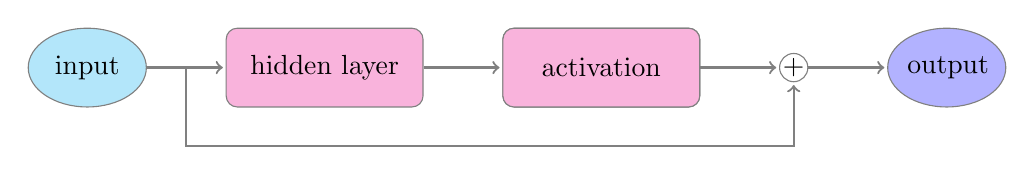
\begin{tikzpicture}[shorten >=1pt,->,draw=black!50, node distance=\layersep]
		\tikzstyle{every pin edge}=[<-,shorten <=1pt]
		\tikzstyle{input}=[ellipse,draw,rounded corners,fill=cyan!30,minimum height=1cm,minimum width=1.5cm,text width=1cm,text centered,inner sep=0pt]
		\tikzstyle{output}=[ellipse,draw,rounded corners,fill=blue!30,minimum height=1cm,minimum width=1.5cm,text width=1cm,text centered,inner sep=0pt]
		\tikzstyle{hidden}=[draw,rounded corners,fill=magenta!30,minimum height=1cm,minimum width=2.5cm,text width=2.5cm,text centered,inner sep=0pt]
		\tikzstyle{operator}=[circle,draw,minimum size=5pt,text centered,inner sep=0pt]
		
		\node[input] (1) {input};
		\node[hidden] (2) at (1.east) [right=1cm] {hidden layer};
		\node[hidden] (3) at (2.east) [right=1cm] {activation};
		\node[hidden] (3) at (2.east) [right=1cm] {activation};
		\node[operator] (4) at (3.east) [right=1cm] {+};
		\node[output] (5) at (4.east) [right=1cm] {output};
		
		\foreach \i/\j in {1/2,2/3,3/4,4/5}
		\draw[thick,->] (\i.east) -- (\j.west);
		\draw[thick,->] ($(1.east)!.5!(2.west)$) -- +(0,-1) -| (4.south); 
		
	\end{tikzpicture}



\end{document}


